\begin{frame}
    \frametitle{FEniCS coding interlude}
    Again, we look at the Poisson problem
    \begin{align*}
        -\Delta u &= e^{-100(x^2 + y^2)} \quad \text{in } \Omega \\
                u &= 0 \quad \text{on } \partial \Omega \\
    \end{align*}
    \vspace{-3em}
    \begin{columns}[c]
        \begin{column}{0.5\textwidth}
    Our mission is to implement the classical, residual-based error
    estimator and to solve this problem adaptively for a given
    tolerance $TOL=1.0e-3$. As marking strategy we choose to mark
    those $30 \%$ of elements with the largest element residual.
        \end{column}
        \begin{column}{0.5\textwidth}
    \begin{center}
        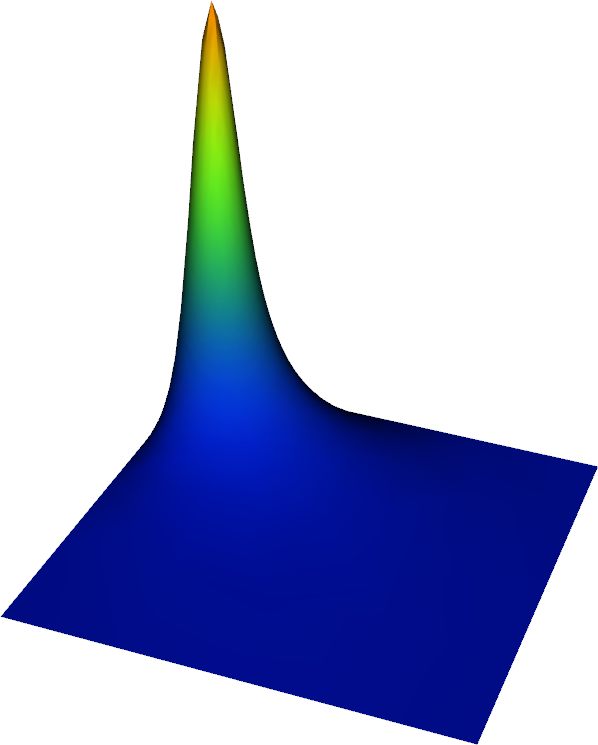
\includegraphics[width=0.8\textwidth]{png/solution-refinement-3.png}
    \end{center}
        \end{column}
    \end{columns}
\end{frame}
